
As described in Section \ref{sec:coding} it is necessary to discover the exact
linear relationship between \gls{ANN} activations and \gls{SNN} activations.
Figure \ref{fig:spike_rates} plots the spike count and spike rate against the
constant input current, using the neuron parameters from Table \ref{tab:neuron_parameters}.

\begin{figure}
  \centering
  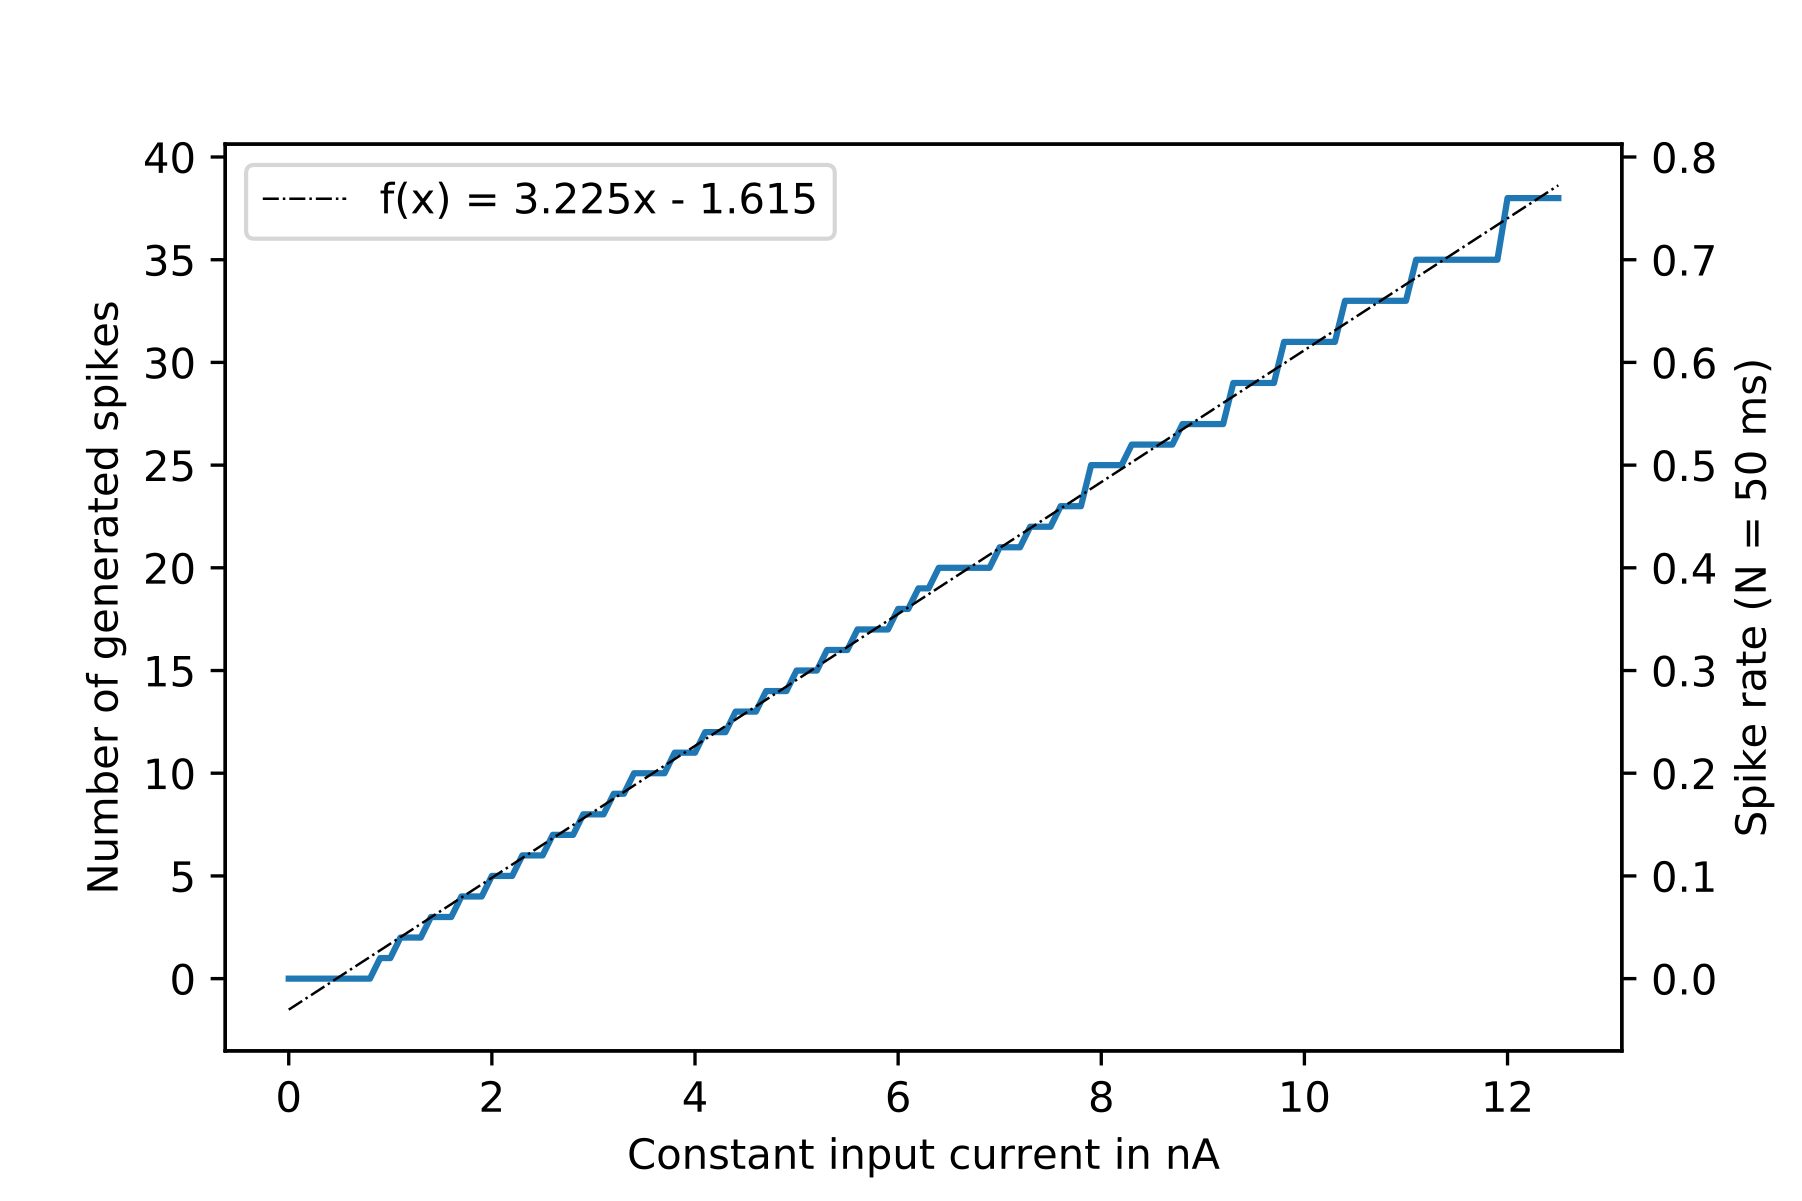
\includegraphics[width=\textwidth]{images/spike_rate.png}
  \caption{Spike count and spike rates in a single neuron simulated over 50 ms.
  A linear regression ($r^2$ = 0.9977) shows the best-fit linear model.}
  \label{fig:spike_rates}
\end{figure}

The relationship shows that there is an approximated linear correlation, when the
input current is kept below 12 and above 1.
Outside this range the relationship becomes unstable: towards 0 it flatlines and
produces no spikes, and towards and beyond 12 it begins to resemble a non-differentiable 
step function.

To illustrate this point in a deeper network, Figure \ref{fig:spike_rates2} shows
a deeper network where three populations of a single neurons are chained.
The weights have been adjusted using an approximation of the weight normalisation scheme
from \textcite{Rueckauer2017}, shown in Equation \ref{eq:weight_norm}.
The approximation assumes that all biases are 0 and weights are 1, such that
the `pure' activation is the input current, shown in the x axis.

\begin{figure}
  \centering
  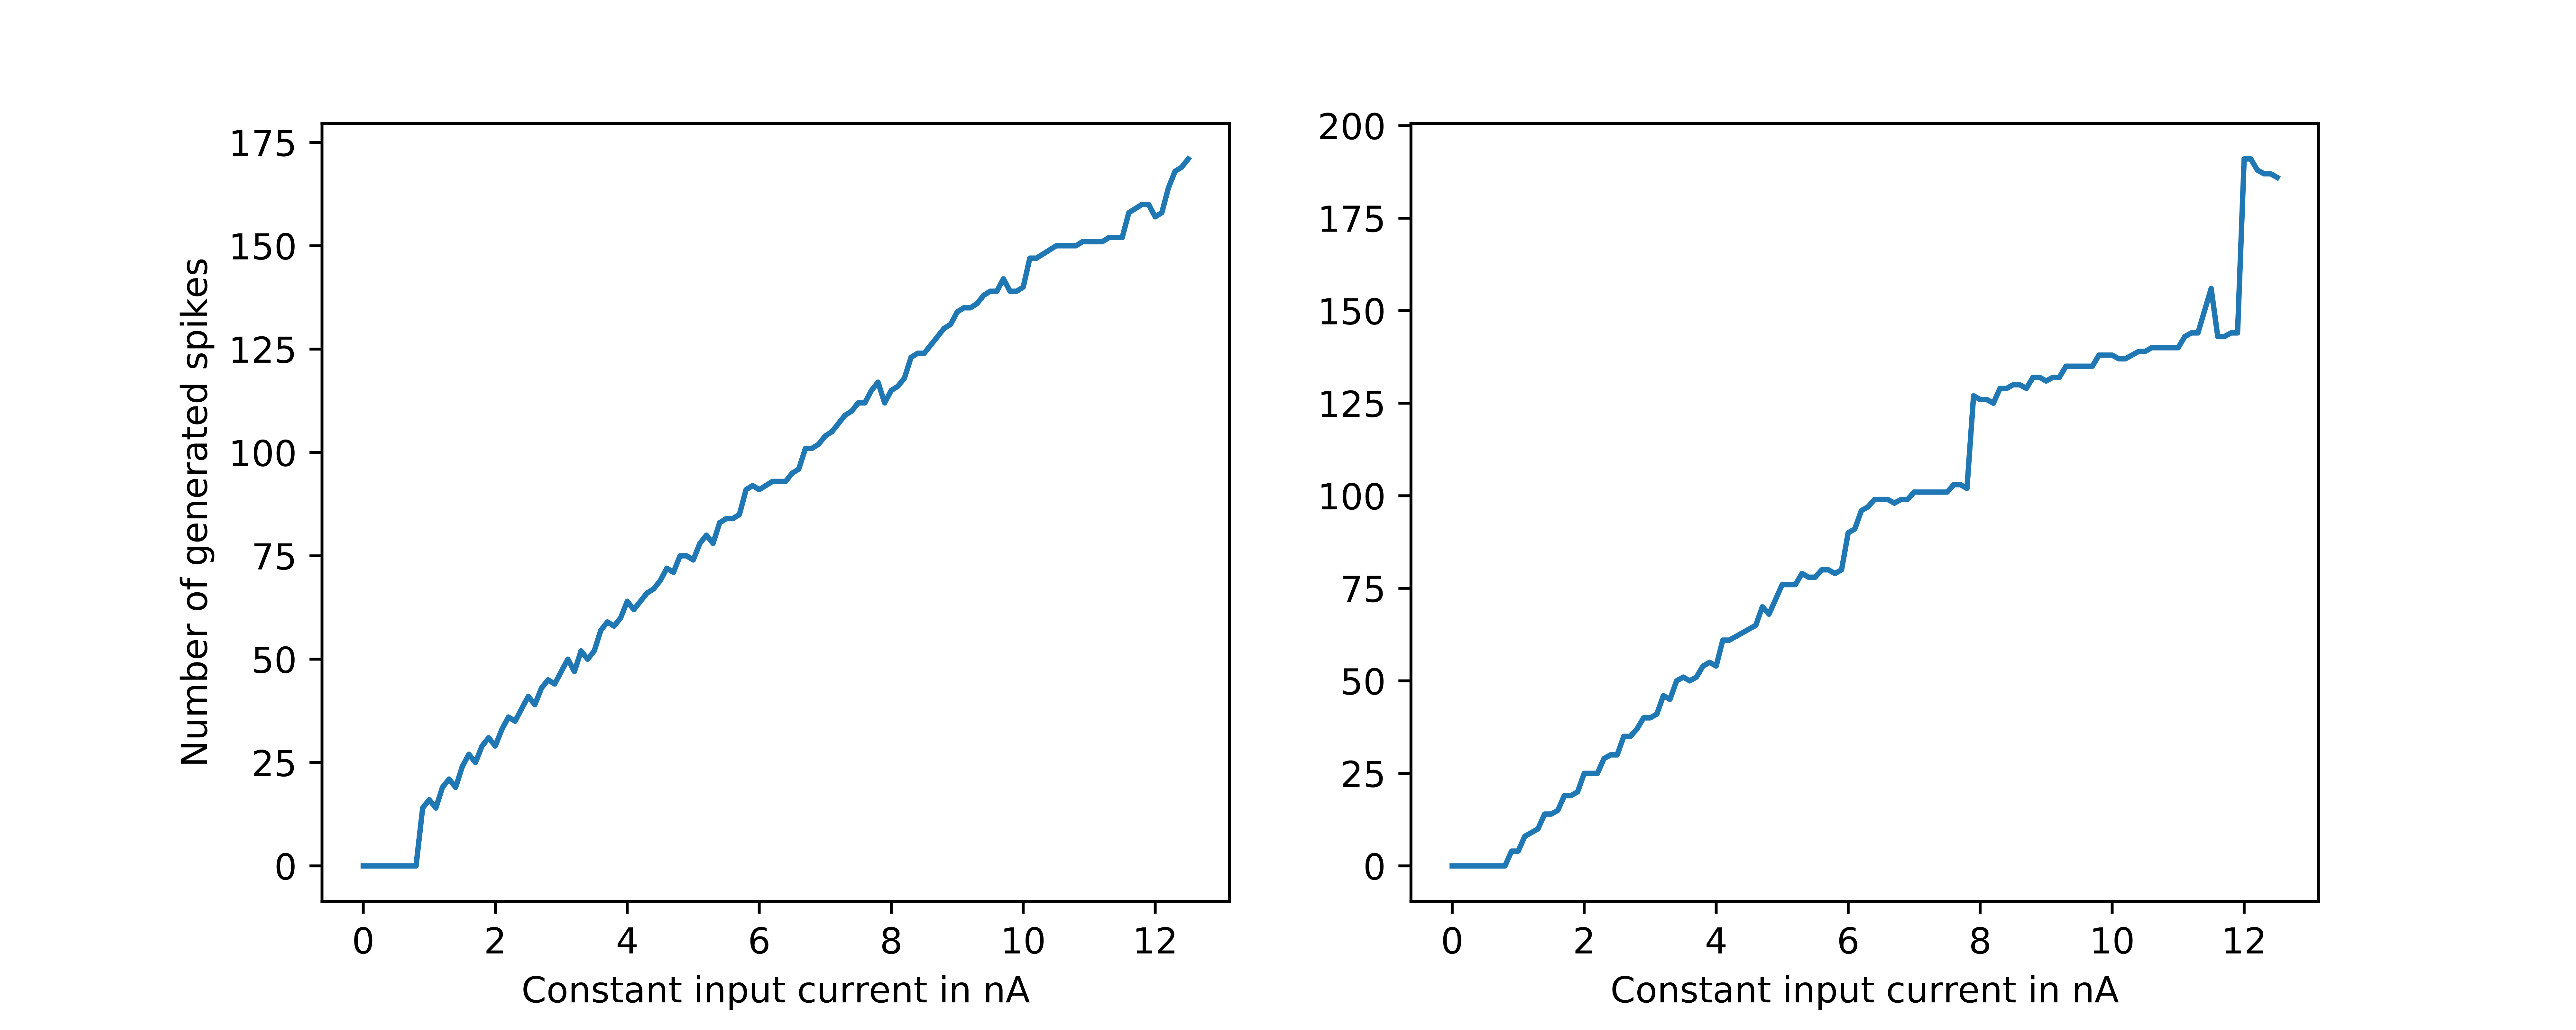
\includegraphics[width=\textwidth]{images/spike_rate2.png}
  \caption{Spike count for second and third population in a chained network of
  single-neuron populations, adjusted for previous neuron activation.}
  \label{fig:spike_rates2}
\end{figure}

The code for the above modelling and representations are available in Appendix
\ref{app:verification}.
